% Provenance (never printed): old terminale S material on the transformation of
% rocks in mountain belts and subduction zones (pressure, temperature, index
% minerals and the Al2SiO5 polymorphs, foliation, contact and regional
% metamorphism). Owner (Sync 0): metamorphism, lithostatic pressure, polymorph,
% index mineral/isograd/metamorphic grade, foliation/schistosity, contact and
% regional metamorphism/aureole. Blueschist and eclogite are g11.06's, the
% geotherm g11.03's, minerals and silicates g11.07's, the rock families, marble
% and slate Book 1's (g6), pressure physics': recalled, never redefined. The
% P-T diagram: figdata/grade-12/al2sio5.py (Holdaway and Mukhopadhyay 1993,
% Table 11; geotherms from Earle 7.3).
\chapter{Les roches métamorphiques}\label{ch:g12:metamorphic-rocks}

Une couche de boue se dépose sur un fond marin et durcit en argilite.
Enfouie à quelques kilomètres et comprimée, elle devient une ardoise, une
roche qui se débite en feuillets minces et plats, ceux d'un toit. Enfouie
plus profond, là où il fait plus chaud, ses minuscules paillettes
grandissent en micas scintillants, parmi lesquels gonflent des grenats
rouges~: c'est un schiste. Plus profond et plus chaud encore, ses minéraux
se rangent en bandes claires et sombres~: c'est un gneiss. Rien n'a fondu
en chemin. La même boue, avec les mêmes éléments chimiques, a simplement
reconstruit ses minéraux pour les accorder au lieu où elle se trouvait.
Lus dans l'autre sens, les minéraux d'une roche métamorphique enregistrent
la profondeur et la chaleur de ce lieu, et ce chapitre apprend à les lire.
% ledger: earle:foliation, earle:settings

\begin{recall}
Les roches se rangent en trois familles --- magmatiques, sédimentaires,
métamorphiques --- et le cycle des roches transforme l'une en l'autre~; le
marbre se forme à partir du calcaire et l'ardoise à partir de l'argilite,
sans fusion (livre~1, année~6). Un minéral est un solide naturel de
composition chimique définie, aux atomes disposés de façon ordonnée~; la
plupart des minéraux de la croûte sont des \omterm{def:g11:minerals:silicate}{silicates}
(\cref{ch:g11:minerals}). Un \omterm{def:g11:lithosphere-asthenosphere:geotherm}{géotherme} est la courbe de la température en
fonction de la profondeur sous un lieu~; près de la surface, la température
augmente de 25 à \qty{30}{\celsius} par kilomètre
(\cref{ch:g11:lithosphere-asthenosphere}). Dans une \omterm{def:g11:subduction-zones:subduction}{zone de subduction}, la
\omterm{def:g11:ocean-ridges:oceanic-lithosphere}{croûte océanique} entraînée vers le bas tout en restant froide se transforme
en \omterm{def:g11:subduction-zones:eclogite}{schiste bleu}, puis en \omterm{def:g11:subduction-zones:eclogite}{éclogite} (\cref{ch:g11:subduction-zones}). La
pression est une force divisée par la surface sur laquelle elle s'exerce~;
elle se mesure en pascals, \qty{1}{Pa} = \qty{1}{N/m^2}.
\end{recall}
% ledger: usgs:metamorphic (Book 1 row), webmineral:formulas, earle:settings, earle:controls

\section{Transformée à l'état solide}

\begin{definition}[Métamorphisme]\label{def:g12:metamorphic-rocks:metamorphism}
Le \emph{métamorphisme}\index{metamorphisme@métamorphisme} est la
transformation des minéraux et de la \omterm{def:g11:igneous-rocks:texture}{texture} d'une roche, à l'état solide,
quand elle est portée à une température et à une pression différentes de
celles sous lesquelles elle s'est formée. La roche qu'elle devient est une
roche métamorphique.
\end{definition}
% ledger: tulane:metamorphism, earle:controls

La roche dont part le \omterm{def:g12:metamorphic-rocks:metamorphism}{métamorphisme} est sa roche mère, le même mot que pour
la roche située sous un sol (\cref{ch:g10:soil-formation}). Le
\omterm{def:g12:metamorphic-rocks:metamorphism}{métamorphisme} commence vers \qty{200}{\celsius}~; au-dessous, les lentes
transformations d'un sédiment enfoui relèvent de son durcissement en roche.
Il s'arrête là où la roche commence à fondre~: à partir de là, ce qui se
passe est magmatique. Entre ces limites, chaque minéral n'est stable que
dans un certain domaine de température et de pression. La plupart des
\omterm{def:g10:soil-formation:clay}{minéraux argileux}, par exemple, ne subsistent que jusque vers 150 ou
\qty{200}{\celsius}~; au-delà, ils se transforment en micas. Quand les
conditions changent, les atomes des minéraux instables se réarrangent, grain
par grain, en minéraux stables dans les nouvelles conditions.
% ledger: tulane:metamorphism, earle:controls

Quatre facteurs décident du résultat. La \textbf{roche mère} fournit les
éléments chimiques~: un calcaire fait uniquement de calcite ne peut devenir
qu'un marbre fait de calcite. La \textbf{température} et la
\textbf{pression} décident des minéraux stables. Et l'\textbf{eau}, présente
en petites quantités entre les grains, transporte des ions dissous d'un
grain à l'autre et accélère les réactions. Le \omterm{def:g12:metamorphic-rocks:metamorphism}{métamorphisme} est lent~: les
nouveaux minéraux grandissent d'environ un millimètre en un million
d'années. Les événements tectoniques qui enfouissent les roches sont lents
eux aussi~: les réactions ont donc en général le temps de se faire.
% ledger: earle:controls

\subsection{Le poids des roches situées au-dessus}

Une roche enfouie à une profondeur $z$ porte le poids de toute la roche
située au-dessus d'elle.

\begin{definition}[Pression lithostatique]\label{def:g12:metamorphic-rocks:lithostatic}
La \emph{pression lithostatique}\index{pression lithostatique} à une
profondeur $z$ est la pression exercée sur une roche par le poids de la
colonne de roches située au-dessus d'elle. Elle est la même dans toutes les
directions.
\end{definition}
% ledger: earle:controls (confining pressure, equal in all directions), tulane:metamorphism

\begin{proposition}[Pression lithostatique]\label{prop:g12:metamorphic-rocks:lithostatic}
Sous une colonne de roches de masse volumique uniforme $\rho$, la \omterm{def:g12:metamorphic-rocks:lithostatic}{pression
lithostatique} à la profondeur $z$ vaut
\[
  P = \rho g z ,
\]
où $g$ est l'accélération de la pesanteur~; on néglige la pression de
l'atmosphère, environ \qty{0.1}{MPa}.
\end{proposition}

\begin{proof}
Prenons une colonne verticale de roches de section horizontale $A$, de la
surface jusqu'à la profondeur $z$. Son volume vaut $Az$, sa masse
$\rho A z$, et son poids $\rho A z g$. Ce poids repose sur la surface $A$
du bas de la colonne~: la pression y vaut donc
$P = \rho A z g / A = \rho g z$.
\end{proof}

Avec la masse volumique moyenne de la \omterm{def:g12:continental-crust:continental-crust}{croûte continentale},
$\rho = \qty{2830}{kg/m^3}$, et $g = \qty{9.81}{m/s^2}$, la pression
augmente de $\rho g = 2830 \times 9.81
\approx \qty{27800}{Pa}$ par mètre, soit environ \qty{27.8}{MPa} par
kilomètre. À la base d'une croûte épaisse de \qty{35}{km}, elle atteint
\[
  P = 2830 \times 9.81 \times \num{35000} \approx \qty{9.7e8}{Pa} \approx
  \qty{0.97}{GPa},
\]
environ \qty{1}{GPa}~: près de dix mille fois la pression de l'atmosphère
au niveau de la mer. On lit souvent les pressions dans l'autre sens, comme
des profondeurs~: \qty{1}{GPa} est atteint à
$\num{e9}/(2830 \times 9.81) \approx \qty{36}{km}$ de profondeur.
% values: P_35km_gpa 0.97168, dPdz_mpa_per_km 27.762, z_1gpa_km 36.02 (al2sio5.py)
% ledger: cm95:crust; Book 1: ussa76:sea-level (101 325 Pa, g0 = 9.80665 m/s2)

Le poids des roches presse de la même façon de tous les côtés. Dans une
chaîne de montagnes, les plaques ajoutent une poussée dans une direction~:
la roche est comprimée plus fort par les côtés que par le haut. Cette
pression \emph{orientée} ne change pas les minéraux stables, mais elle
change leur disposition, comme le montre la
\cref{sec:g12:metamorphic-rocks:foliation}.
% ledger: earle:controls (directed pressure), earle:foliation

\section{Minéraux index et degré métamorphique}

\subsection{Trois minéraux pour une seule formule}

\begin{definition}[Polymorphe]\label{def:g12:metamorphic-rocks:polymorph}
Deux minéraux sont des \emph{polymorphes}\index{polymorphe} quand ils ont la
même composition chimique mais des structures cristallines différentes~:
les mêmes atomes, disposés autrement.
\end{definition}
% ledger: earle:controls

Trois minéraux ont la formule \ce{Al2SiO5}~: le disthène, l'andalousite et
la sillimanite. Chacun est stable dans son propre domaine de température et
de pression, mesuré en laboratoire en maintenant des cristaux à une
température et à une pression choisies et en observant quel \omterm{def:g12:metamorphic-rocks:polymorph}{polymorphe}
grandit aux dépens de l'autre. Le disthène est le plus dense des trois,
\qty{3.61}{g/cm^3} contre \qty{3.24}{g/cm^3} pour la sillimanite et
\qty{3.15}{g/cm^3} pour l'andalousite~: ses atomes sont plus serrés, et
c'est lui que les hautes pressions favorisent.
% ledger: earle:controls, hm93:triple, hm93:table11; Book 3: webmineral:polymorphs (densities)

\begin{omfigure}
\begin{tikzpicture}
\begin{axis}[omrecord, name=pt, scale only axis, width=0.62\linewidth, height=6.4cm,
  xmin=200, xmax=900, ymin=0, ymax=1.2, y dir=reverse,
  xlabel={température (\unit{\celsius})}, ylabel={pression (\unit{GPa})},
  xtick={200,300,...,900}, ytick={0,0.2,...,1.2},
  yticklabel style={/pgf/number format/fixed, /pgf/number format/precision=1},
  axis y line*=left]
% computed in figdata/grade-12/al2sio5.py from Holdaway and Mukhopadhyay (1993), Table 11
\addplot[omDef, line width=0.9pt, densely dashed] table[x=T10, y=P_GPa] {figdata/out/grade-12-al2sio5-geotherms.dat};
\addplot[omMeth, line width=0.9pt, densely dashed] table[x=T30, y=P_GPa] {figdata/out/grade-12-al2sio5-geotherms.dat};
\addplot[omThm, line width=0.9pt, densely dashed] table[x=T50, y=P_GPa] {figdata/out/grade-12-al2sio5-geotherms.dat};
\addplot[black, line width=1.2pt] table[x=T, y=P_GPa] {figdata/out/grade-12-al2sio5-andky.dat};
\addplot[black, line width=1.2pt] table[x=T, y=P_GPa] {figdata/out/grade-12-al2sio5-kysil.dat};
\addplot[black, line width=1.2pt] table[x=T, y=P_GPa] {figdata/out/grade-12-al2sio5-andsil.dat};
\addplot[black, line width=1.2pt, dotted] table[x=T, y=P_GPa] {figdata/out/grade-12-al2sio5-andsilx.dat};
\addplot[only marks, mark=*, mark size=2pt, black] coordinates {(504.2,0.3758)};
\addplot[only marks, mark=o, mark size=2pt, line width=0.8pt, black] coordinates {(573.6,0.5216) (340.1,0.1833) (553.0,0.3015)};
\coordinate (ky) at (axis cs:370,0.55);
\coordinate (and) at (axis cs:470,0.12);
\coordinate (sil) at (axis cs:765,0.57);
\coordinate (tp) at (axis cs:504.2,0.3758);
\coordinate (g10) at (axis cs:415,1.0);
\coordinate (g30) at (axis cs:206,0.36);
\coordinate (g50) at (axis cs:895,0.355);
\end{axis}
\begin{axis}[scale only axis, width=0.62\linewidth, height=6.4cm, at={(pt.south west)}, anchor=south west,
  xmin=200, xmax=900, ymin=0, ymax=43.224, y dir=reverse, axis x line=none, axis y line*=right,
  axis line style={-}, ylabel={profondeur (\unit{km})}, ytick={0,5,...,40},
  every axis label/.append style={font=\small}, tick label style={font=\small}]
\end{axis}
\node[font=\small\bfseries] at (ky) {disthène};
\node[font=\small\bfseries] at (and) {andalousite};
\node[font=\small\bfseries] at (sil) {sillimanite};
\node[font=\scriptsize, text=omDef, anchor=west, inner sep=1pt] at (g10) {\qty{10}{\celsius/km}, zone de subduction};
\node[font=\scriptsize, text=omMeth!70!black, anchor=north west, inner sep=1pt, align=left] at (g30) {\qty{30}{\celsius/km},\\typique};
\node[font=\scriptsize, text=omThm, anchor=south east, inner sep=1pt] at (g50) {\qty{50}{\celsius/km}, région volcanique};
\end{tikzpicture}

{\small Les domaines des trois \omterm{def:g12:metamorphic-rocks:polymorph}{polymorphes} de \ce{Al2SiO5}, la pression
croissant vers le bas comme la profondeur (échelle de droite, pour une
croûte de masse volumique \qty{2830}{kg/m^3}). Traits noirs~: les limites
mesurées en laboratoire~; les trois se rejoignent au point triple (point
noir), à \qty{504}{\celsius} et \qty{0.375}{GPa}. En tirets~: trois
\omterm{def:g11:lithosphere-asthenosphere:geotherm}{géothermes}, partant de \qty{10}{\celsius} en surface~; les cercles marquent
l'endroit où ils croisent une limite.}
\end{omfigure}
% values: triple_T 504.21, triple_P_gpa 0.37584, triple_z_km 13.538; crossings 30: 573.6 degC 18.79 km; 50: 340.1 degC 6.60 km, 553.0 degC 10.86 km (al2sio5.py)
% ledger: hm93:table11, hm93:triple, cm95:crust, earle:settings

Le diagramme est une carte de stabilité. Chaque point est une température
et une pression~; chaque domaine est celui du \omterm{def:g12:metamorphic-rocks:polymorph}{polymorphe} stable en ce point.
Le disthène occupe les hautes pressions, l'andalousite les basses pressions
et les températures modérées, la sillimanite les hautes températures. Le
long d'une limite, deux \omterm{def:g12:metamorphic-rocks:polymorph}{polymorphes} sont également stables, et au point
triple, les trois. Les limites ne sont pas connues exactement~: le point
triple est incertain d'environ \qty{20}{\celsius} et \qty{0.025}{GPa}, et
des traces de fer dans les cristaux déplacent la limite
andalousite--sillimanite de jusqu'à \qty{20}{\celsius}.
% ledger: hm93:triple

\begin{method}[Lire un diagramme pression--température]\label{met:g12:metamorphic-rocks:pt}
\begin{enumerate}
  \item Placer le point de la roche~: sa température sur l'axe horizontal,
        sa pression sur l'axe vertical.
  \item Lire le domaine où il tombe~: celui du minéral stable en ce point.
  \item Convertir la pression en profondeur avec $z = P/(\rho g)$, ou lire
        celle-ci sur l'échelle des profondeurs.
  \item Pour un minéral trouvé dans une roche, lire dans l'autre sens~: la
        roche se trouvait dans le domaine de ce minéral quand elle a
        cristallisé. Deux minéraux formés ensemble, ou un minéral absent,
        resserrent encore l'intervalle.
\end{enumerate}
\end{method}

\begin{example}[La limite disthène--sillimanite]\label{ex:g12:metamorphic-rocks:kysil}
À \qty{0.6}{GPa}, le disthène se transforme en sillimanite vers
\qty{611}{\celsius}. Cette pression est atteinte à $z = \num{0.6e9} / (2830
\times 9.81) \approx \qty{21.6}{km}$. Entre 600 et \qty{700}{\celsius}, la
limite monte de \qty{0.209}{GPa}, soit $0.209/0.0278 \approx
\qty{7.5}{km}$ de profondeur~: une roche située \qty{7.5}{km} plus bas doit
être environ \qty{100}{\celsius} plus chaude pour se transformer en
sillimanite. Un schiste qui contient du disthène mais pas de sillimanite,
et qui a cristallisé à \qty{21.6}{km}, était donc plus froid qu'environ
\qty{611}{\celsius}.
\end{example}
% values: kysil_T_at_6kbar 611, kysil_z_at_6kbar 21.612, kysil_slope 2.09 kbar per 100 degC, dPdz 27.762 MPa/km (al2sio5.py)

\subsection{Minéraux index et isogrades}

Dans une bande de roches qui étaient toutes au départ la même boue, les
minéraux changent d'un endroit à l'autre, parce que les roches n'ont pas
toutes été enfouies aussi profond ni chauffées autant.

\begin{definition}[Minéral index~; isograde~; degré métamorphique]\label{def:g12:metamorphic-rocks:index-mineral}
Le \emph{degré métamorphique}\index{degre metamorphique@degré métamorphique}
d'une roche est l'intensité du \omterm{def:g12:metamorphic-rocks:metamorphism}{métamorphisme} qu'elle a subi, fixée par la
température et la pression qu'elle a atteintes. Un \emph{minéral
index}\index{mineral index@minéral index} est un minéral dont la première
apparition, dans des roches de même composition d'origine, marque un degré
donné. Une \emph{isograde}\index{isograde} est la ligne d'une carte (une
surface dans le sous-sol) qui joint les lieux où un minéral index apparaît
pour la première fois~: le long de cette ligne, les roches ont atteint le
même degré.
\end{definition}
% ledger: tulane:metamorphism, earle:regional

Les roches issues d'une boue, riches en aluminium, montrent la suite la plus
nette. À mesure que le degré augmente, les \omterm{def:g12:metamorphic-rocks:index-mineral}{minéraux index} apparaissent dans
l'ordre chlorite, biotite, grenat, staurotide, disthène, sillimanite, et
les terrains qu'ils séparent s'appellent zone à chlorite, zone à biotite,
et ainsi de suite. Température et pression augmentent toutes deux le long de
cette suite, comme dans une croûte épaissie sous une chaîne de montagnes.
% ledger: iugs:barrow, earle:regional

\begin{omfigure}
\begin{tikzpicture}[font=\scriptsize]
  \def\zone#1#2#3#4{\fill[#1] (#2,0) ellipse ({#3} and {#4});}
  \zone{omProp!8}{0}{6.6}{2.55}
  \zone{omProp!18}{0.5}{5.4}{2.2}
  \zone{omProp!32}{1.0}{4.3}{1.82}
  \zone{omThm!28}{1.4}{3.2}{1.44}
  \zone{omThm!45}{1.8}{2.1}{1.06}
  \zone{omThm!65}{2.2}{1.0}{0.66}
  \foreach \c/\a/\b in {0.5/5.4/2.2, 1.0/4.3/1.82, 1.4/3.2/1.44, 1.8/2.1/1.06, 2.2/1.0/0.66}
    \draw[black!70, line width=0.6pt] (\c,0) ellipse ({\a} and {\b});
  \draw[black!40] (0,0) ellipse (6.6 and 2.55);
  \node at (-5.75,0) {chlorite};
  \node at (-4.1,0) {biotite};
  \node at (-2.55,0) {grenat};
  \node at (-1.05,0) {staurotide};
  \node at (0.45,0) {disthène};
  \node[text=white, font=\scriptsize\bfseries] at (2.2,0) {sillimanite};
  \draw[omDef, -{Stealth}, line width=0.8pt] (5.6,-2.6) node[right, text=omDef] {degré croissant} -- (3.0,-0.65);
  \draw[black!70] (3.76,1.394) -- (5.8,2.2) node[right, align=left] {isograde\\du grenat};
\end{tikzpicture}

{\small Carte schématique de zones métamorphiques dans des roches issues
d'une boue~: chaque \omterm{def:g12:metamorphic-rocks:index-mineral}{isograde} (trait noir) marque la première apparition d'un
\omterm{def:g12:metamorphic-rocks:index-mineral}{minéral index}, et le degré augmente vers le cœur de la chaîne, là où les
roches ont été enfouies le plus profond et chauffées le plus. Les zones
réelles sont déformées et recoupées par des \omterm{def:g12:mountain-building:fold}{plis} et des failles~; leurs
largeurs sont ici arbitraires.}
\end{omfigure}
% ledger: iugs:barrow, earle:regional

\begin{history}[Les zones de Barrow]
Dans les années 1890, le géologue George Barrow cartographia les schistes et
les gneiss des Highlands d'Écosse et remarqua que leurs minéraux changeaient
à travers la région dans un ordre régulier. Il fut le premier à diviser une
région en zones d'après les minéraux que contiennent ses roches. Son nom est
resté attaché à la suite~: on dit des roches qui la suivent qu'elles
montrent un \omterm{def:g12:metamorphic-rocks:metamorphism}{métamorphisme} \emph{barrovien}.
\end{history}
% ledger: earle:regional, barrow1893:paper, iugs:barrow

On peut aussi juger grossièrement du degré d'après la seule température.
Les roches chauffées de 150 à \qty{300}{\celsius} sont de très faible
degré, de 300 à \qty{450}{\celsius} de faible degré, de 450 à
\qty{550}{\celsius} de degré moyen, et au-delà de \qty{550}{\celsius} de
haut degré. À faible degré, les roches sont riches en minéraux qui
contiennent de l'eau dans leur structure, comme les argiles et la
chlorite~; à mesure que le degré augmente, elles perdent cette eau.
% ledger: earle:foliation (Table 7.1 grades), tulane:metamorphism

\section{La foliation}\label{sec:g12:metamorphic-rocks:foliation}

Comprimés pendant qu'ils grandissent, les minéraux ne grandissent pas dans
toutes les directions. Les grains plats comme les micas, et les grains
allongés comme les amphiboles, cristallisent avec leurs faces plates ou
leurs grands axes en travers de la direction de la poussée~; les grains déjà
présents sont aplatis de la même façon.
% ledger: earle:foliation, tulane:metamorphism

\begin{definition}[Foliation~; schistosité]\label{def:g12:metamorphic-rocks:foliation}
Une \emph{foliation}\index{foliation} est un ensemble de plans parallèles
dans une roche métamorphique, dû à l'alignement de ses minéraux plats ou
allongés~; la roche se débite le plus facilement le long de ces plans. La
\emph{schistosité}\index{schistosite@schistosité} est la foliation d'un
schiste, dont les cristaux de mica alignés sont assez grands pour être vus.
\end{definition}
% ledger: earle:foliation, tulane:metamorphism

\begin{omfigure}
\begin{tikzpicture}[font=\scriptsize]
  \pgfmathsetseed{4}
  % before: random flakes in a square
  \draw[black!60, fill=omLithShale!35] (0,0) rectangle (3.2,3.2);
  \foreach \i in {1,...,38} {
    \pgfmathsetmacro{\x}{0.3+2.6*rnd}\pgfmathsetmacro{\y}{0.3+2.6*rnd}\pgfmathsetmacro{\a}{180*rnd}
    \draw[black!75, line width=1.1pt] ($(\x,\y)+(\a:0.2)$) -- ($(\x,\y)+(\a+180:0.2)$);
  }
  \foreach \i in {1,...,14} {
    \pgfmathsetmacro{\x}{0.3+2.6*rnd}\pgfmathsetmacro{\y}{0.3+2.6*rnd}
    \fill[white, draw=black!40] (\x,\y) circle (0.07);
  }
  \node[below] at (1.6,-0.3) {avant~: paillettes dans tous les sens};
  % after: squeezed from the sides
  \begin{scope}[xshift=7.3cm]
  \draw[black!60, fill=omLithSchist!45] (0,-0.3) rectangle (2.4,3.5);
  \foreach \i in {1,...,38} {
    \pgfmathsetmacro{\x}{0.2+2.0*rnd}\pgfmathsetmacro{\y}{0.1+3.0*rnd}\pgfmathsetmacro{\a}{90+12*(rnd-0.5)}
    \draw[black!75, line width=1.1pt] ($(\x,\y)+(\a:0.24)$) -- ($(\x,\y)+(\a+180:0.24)$);
  }
  \foreach \i in {1,...,14} {
    \pgfmathsetmacro{\x}{0.2+2.0*rnd}\pgfmathsetmacro{\y}{0.1+3.0*rnd}
    \fill[white, draw=black!40] (\x,\y) ellipse (0.045 and 0.09);
  }
  \draw[omThm, -{Stealth}, line width=1.4pt] (-1.1,1.6) -- (-0.15,1.6);
  \draw[omThm, -{Stealth}, line width=1.4pt] (3.5,1.6) -- (2.55,1.6);
  \node[below] at (1.2,-0.3) {après~: paillettes en travers de la poussée};
  \node[omThm, above] at (-0.65,1.65) {poussée};
  \node[omThm, above] at (3.05,1.65) {poussée};
  \end{scope}
  \draw[-{Stealth}, black!50, line width=0.8pt] (3.5,1.6) -- node[above] {chauffée et} node[below] {comprimée} (5.2,1.6);
\end{tikzpicture}

{\small La formation d'une \omterm{def:g12:metamorphic-rocks:foliation}{foliation}. À gauche~: une boue avec des
paillettes d'argile (en noir) et des grains de quartz (en blanc) orientés
dans tous les sens. À droite~: comprimée par les côtés pendant qu'elle est
chauffée, la roche fait pousser des paillettes de mica en travers de la
poussée et aplatit ses grains~: elle se débite désormais selon des plans
verticaux.}
\end{omfigure}
% ledger: earle:foliation

La boue, riche en paillettes plates d'argile, montre le mieux la suite. À
mesure que le degré augmente, elle devient tour à tour~:
\begin{itemize}
  \item une \textbf{ardoise}, dont les paillettes alignées d'argile et de
        mica sont trop petites pour être vues~; elle se débite en feuillets
        plats~;
  \item un \textbf{phyllade}, dont les micas ont assez grandi pour lui
        donner un \omterm{def:g11:minerals:lustre}{éclat} soyeux~;
  \item un \textbf{schiste}, dont les micas sont visibles, souvent avec de
        plus gros cristaux de grenat, de disthène ou de staurotide parmi
        eux~;
  \item un \textbf{gneiss}, dont les minéraux se sont séparés en bandes
        claires (quartz, feldspath) et en bandes sombres, et qui contient
        peu de mica, voire pas du tout, car il fait trop chaud pour qu'il
        subsiste.
\end{itemize}
% ledger: earle:foliation, earle:settings (slate 5-10 km to gneiss 20-25 km on a typical gradient)

\begin{omfigure}
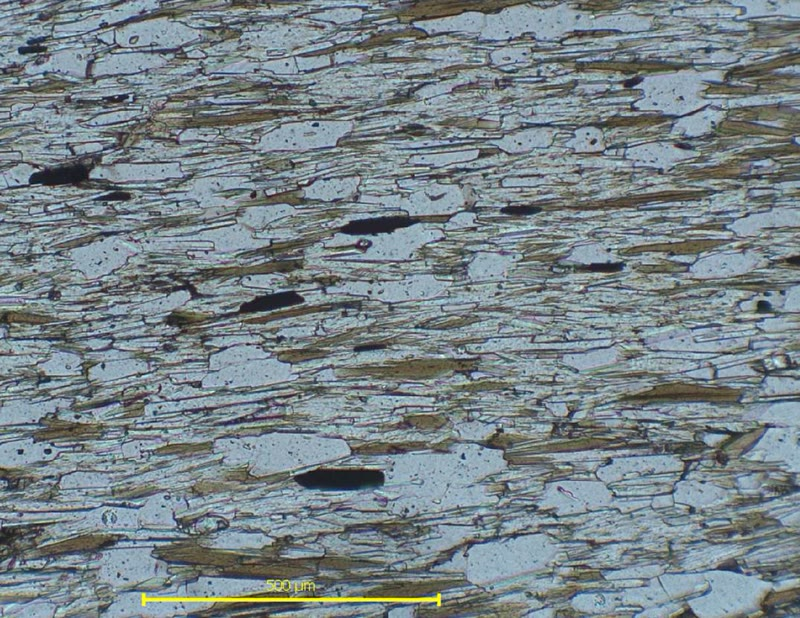
\includegraphics[height=4.3cm]{images/book2/g12-geoloshe-slaty-cleavage.jpg}\hspace{0.03\linewidth}%
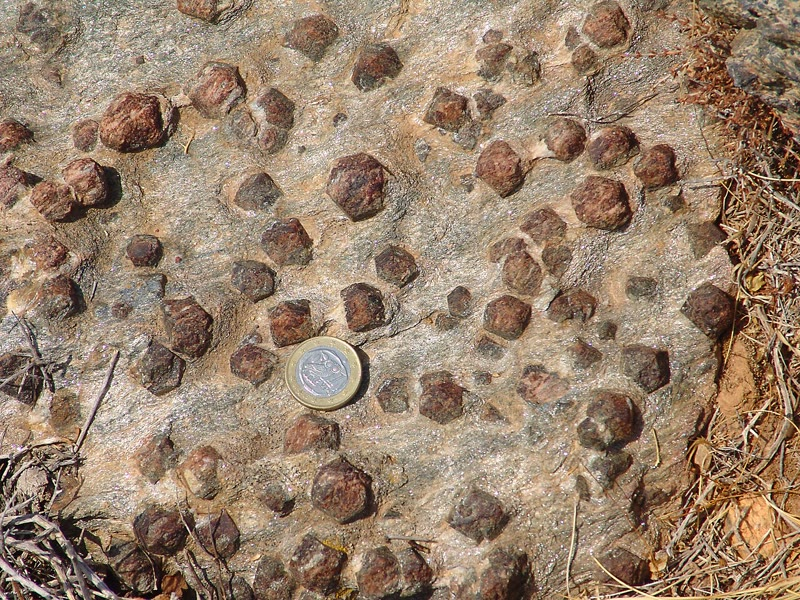
\includegraphics[height=4.3cm]{images/book2/g12-churchard-syros-garnet-schist.jpg}

\smallskip
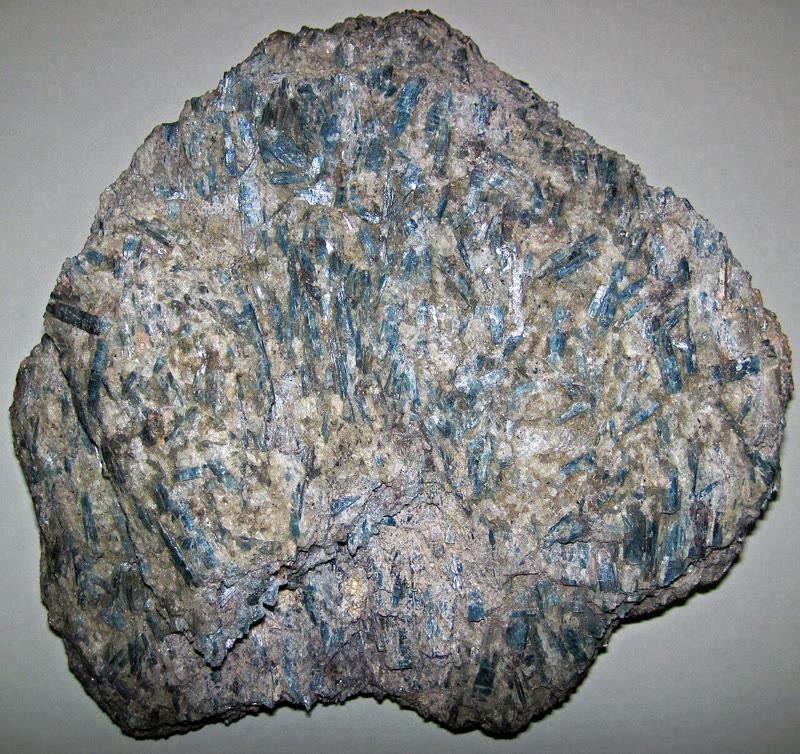
\includegraphics[height=4.3cm]{images/book2/g12-stjohn-kyanite-schist.jpg}\hspace{0.03\linewidth}%
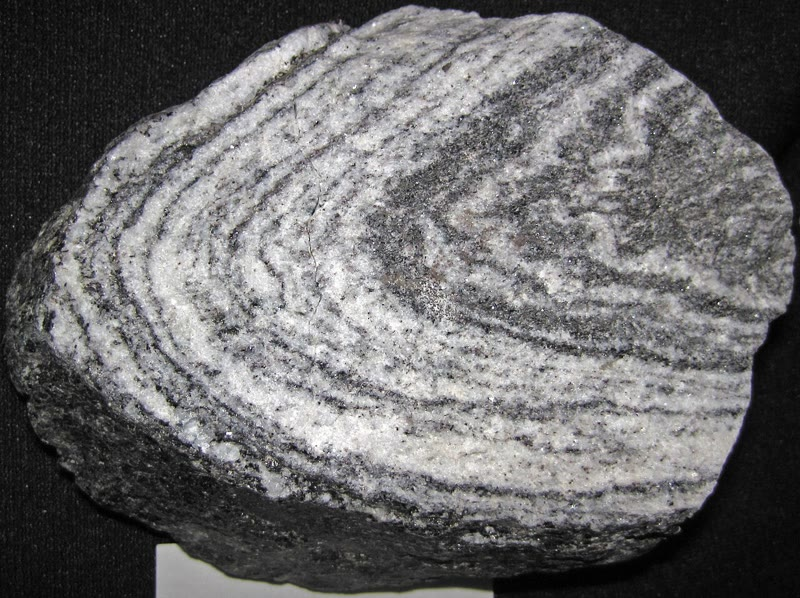
\includegraphics[height=4.3cm]{images/book2/g12-stjohn-gneiss.jpg}

{\small En haut à gauche~: une ardoise au microscope (la barre jaune mesure
\qty{500}{\micro\metre})~: ses paillettes de mica sont toutes orientées de
la même façon. En haut à droite~: un micaschiste à grenat de l'île de
Syros~; la pièce mesure \qty{23}{mm} de diamètre. En bas à gauche~: un
schiste à lames bleues de disthène. En bas à droite~: un gneiss à bandes de
quartz (claires) et de mica biotite (sombres). Photographies Geoloshe
(CC0), Graeme Churchard (CC~BY~2.0) et James St.~John (CC~BY~2.0).}
\end{omfigure}
% ledger: photo:g12-slaty-cleavage, photo:g12-syros-schist, photo:g12-kyanite-schist, photo:g12-gneiss

Le long d'un \omterm{def:g11:lithosphere-asthenosphere:geotherm}{géotherme} typique, l'ardoise se forme entre environ 5 et
\qty{10}{km} de profondeur, le phyllade entre 10 et 15, le schiste entre 15
et 20, et le gneiss entre 20 et \qty{25}{km}~; plus profond encore, la
roche commence à fondre par endroits. La \omterm{def:g12:metamorphic-rocks:foliation}{foliation} enregistre la direction
de la compression~: elle se forme en travers du \omterm{def:g12:mountain-building:shortening}{raccourcissement} qui
édifie les montagnes (\cref{ch:g12:mountain-building}), et le litage
d'origine de la boue peut encore se voir, qui la recoupe obliquement.
% ledger: earle:settings, earle:foliation

Les roches dépourvues de minéraux plats ou allongés ne montrent pas de
\omterm{def:g12:metamorphic-rocks:foliation}{foliation}, même quand elles sont comprimées. Un calcaire devient un
\textbf{marbre}, fait de plus gros cristaux de calcite dans lesquels les
fossiles ont été effacés~; un grès devient un \textbf{quartzite}, dont les
grains de quartz ont grandi les uns dans les autres~; et une boue chauffée
sans être comprimée devient une roche dure, à grain fin et sans \omterm{def:g12:metamorphic-rocks:foliation}{foliation},
une \textbf{cornéenne}.
% ledger: earle:foliation, earle:contact

\section{Métamorphisme de contact et métamorphisme régional}

\begin{definition}[Métamorphisme de contact~; métamorphisme régional~; auréole]\label{def:g12:metamorphic-rocks:contact-regional}
Le \emph{métamorphisme de contact}\index{metamorphisme de contact@métamorphisme de contact}
est le \omterm{def:g12:metamorphic-rocks:metamorphism}{métamorphisme} de roches chauffées par un corps de magma qui s'y est
mis en place~; il se limite à une zone autour de l'\omterm{def:g11:igneous-rocks:intrusion}{intrusion}, son
\emph{auréole}\index{aureole@auréole}, dans laquelle le degré augmente vers
le contact. Le \emph{métamorphisme régional}\index{metamorphisme regional@métamorphisme régional}
touche des roches enfouies profondément sur de vastes régions, en général
là où des plaques convergent~; les roches sont comprimées autant que
chauffées, et sont presque toujours foliées.
\end{definition}
% ledger: earle:contact, earle:regional, tulane:metamorphism

\subsection{Autour d'un corps de magma}

Un corps de magma à environ \qty{1000}{\celsius} qui monte dans la croûte
supérieure froide chauffe les roches qui l'entourent. Leur température peut
atteindre de 300 à plus de \qty{800}{\celsius}, sous les faibles pressions
des petites profondeurs. L'\omterm{def:g12:metamorphic-rocks:contact-regional}{auréole} est étroite~: quelques centimètres
autour d'une lame mince de magma, jusqu'à plusieurs dizaines de mètres
autour d'un grand corps. Ses roches sont chauffées sans être comprimées~:
elles ne sont donc pas foliées~; la boue devient cornéenne, le calcaire
marbre, le grès quartzite. Un corps de magma qui se met en place en
profondeur, dans des roches déjà chaudes, ne produit presque pas
d'\omterm{def:g12:metamorphic-rocks:contact-regional}{auréole}.
% ledger: earle:contact, earle:settings (magma bodies around 1000 degC)

\begin{omfigure}
\begin{tikzpicture}[font=\scriptsize]
  \def\pluton{(3.0,0) .. controls (3.0,2.3) and (7.0,2.3) .. (7.0,0) -- cycle}
  \def\aureole{(2.45,0) .. controls (2.45,2.95) and (7.55,2.95) .. (7.55,0) -- cycle}
  \fill[lith sandstone] (0,0) rectangle (10,0.8);
  \fill[lith limestone] (0,0.8) rectangle (10,1.6);
  \fill[lith shale] (0,1.6) rectangle (10,3);
  \fill[omThm, opacity=0.30] \aureole;
  \draw[omThm, line width=0.6pt, dashed] (2.45,0) .. controls (2.45,2.95) and (7.55,2.95) .. (7.55,0);
  \fill[lith granite] \pluton;
  \draw[black!70, line width=0.6pt] (3.0,0) .. controls (3.0,2.3) and (7.0,2.3) .. (7.0,0);
  \draw[black!60] (0,0) rectangle (10,3);
  \node[fill=white, inner sep=1.5pt] at (5,0.45) {granite (ancien magma)};
  \draw[black!70] (6.0,1.95) -- (10.6,2.4) node[right] {cornéenne, issue de la boue};
  \draw[black!70] (7.0,1.2) -- (10.6,1.2) node[right] {marbre, issu du calcaire};
  \draw[black!70] (7.25,0.4) -- (10.6,0.4) node[right] {quartzite, issu du grès};
  \node[left] at (0,2.3) {argilite};
  \node[left] at (0,1.2) {calcaire};
  \node[left] at (0,0.4) {grès};
  \draw[omThm] (4.2,2.05) -- (3.4,3.25) node[above, omThm] {auréole};
\end{tikzpicture}

{\small Le \omterm{def:g12:metamorphic-rocks:contact-regional}{métamorphisme de contact}, en coupe~: un corps de magma est monté
dans des roches sédimentaires litées et a chauffé autour de lui une étroite
\omterm{def:g12:metamorphic-rocks:contact-regional}{auréole} (en rouge), dont les roches recristallisent sans être comprimées.
Schéma~: les \omterm{def:g12:metamorphic-rocks:contact-regional}{auréoles} réelles sont larges de quelques centimètres à
quelques dizaines de mètres.}
\end{omfigure}
% ledger: earle:contact

\subsection{Sous une chaîne de montagnes}

Le \omterm{def:g12:metamorphic-rocks:contact-regional}{métamorphisme régional} demande un enfouissement à 10 ou \qty{20}{km}~:
il touche donc des milliers de kilomètres carrés à la fois. Le lieu le plus
probable est la \omterm{def:g12:continental-crust:root}{racine} d'une chaîne de montagnes, où la collision épaissit
la croûte et pousse ses roches vers le bas
(\cref{ch:g12:mountain-building}). Dans une ancienne chaîne dont les zones
ont été cartographiées, les roches de la zone à sillimanite ont été
chauffées au-delà de \qty{700}{\celsius} et enfouies à 20 à \qty{25}{km} de
profondeur, tandis que celles de la zone externe à chlorite n'ont sans
doute jamais été enfouies à plus de \qty{5}{km} environ. Les montagnes
situées au-dessus ont ensuite été usées pendant des dizaines de millions
d'années~; à mesure que la charge était enlevée, la croûte épaisse est
remontée, et les zones autrefois profondes affleurent aujourd'hui
(\cref{ch:g12:destruction-of-mountains}).
% ledger: earle:regional

\subsection{Trois géothermes}

Les \omterm{def:g12:metamorphic-rocks:polymorph}{polymorphes} montrent d'un coup d'œil que la même profondeur ne donne pas
partout la même roche~: cela dépend du \omterm{def:g11:lithosphere-asthenosphere:geotherm}{géotherme}. La figure des \omterm{def:g12:metamorphic-rocks:polymorph}{polymorphes}
en porte trois.
% ledger: earle:settings

\begin{itemize}
  \item Un \omterm{def:g11:lithosphere-asthenosphere:geotherm}{géotherme} \textbf{typique}, d'environ \qty{30}{\celsius} par
        kilomètre~: la température atteint environ \qty{300}{\celsius} à
        \qty{10}{km}. Il passe sous le point triple~: le disthène cède donc
        directement la place à la sillimanite, vers \qty{574}{\celsius} et
        \qty{18.8}{km}.
  \item Un \omterm{def:g11:lithosphere-asthenosphere:geotherm}{géotherme} de \textbf{région volcanique}, de 40 à
        \qty{50}{\celsius} par kilomètre, raidi par la chaleur du magma qui
        monte~: les roches atteignent de hautes températures à faible
        profondeur. À \qty{50}{\celsius} par kilomètre, l'andalousite
        apparaît vers \qty{6.6}{km} et cède la place à la sillimanite vers
        \qty{10.9}{km}, à \qty{553}{\celsius}.
  \item Le \omterm{def:g11:lithosphere-asthenosphere:geotherm}{géotherme} d'une \textbf{\omterm{def:g11:subduction-zones:subduction}{zone de subduction}}, de moins de
        \qty{10}{\celsius} par kilomètre~: la \omterm{def:g11:ocean-ridges:oceanic-lithosphere}{croûte océanique} entraînée vers
        le bas reste de plusieurs centaines de degrés plus froide que le
        manteau qui l'entoure. À \qty{36}{km}, elle n'est qu'à environ
        \qty{370}{\celsius}, au cœur du domaine du disthène. C'est le chemin
        froid et de haute pression sur lequel le basalte devient \omterm{def:g11:subduction-zones:eclogite}{schiste
        bleu}, puis \omterm{def:g11:subduction-zones:eclogite}{éclogite}, vers \qty{35}{km}.
\end{itemize}
% values: cross_30_0 573.6 degC 18.79 km; cross_50_0 340.1 degC 6.60 km; cross_50_1 553.0 degC 10.86 km; sub10_T_at_1gpa 370.2 (al2sio5.py)
% ledger: earle:settings

Chaque roche métamorphique garde ainsi la trace du \omterm{def:g11:lithosphere-asthenosphere:geotherm}{géotherme} sous lequel
elle s'est formée, et du contexte de plaques qui l'explique~: l'andalousite
et les cornéennes signalent de la chaleur à faible profondeur, autour de
corps de magma~; les schistes et les gneiss à disthène et à sillimanite, les
\omterm{def:g12:continental-crust:root}{racines} profondes des chaînes de montagnes~; les \omterm{def:g11:subduction-zones:eclogite}{schistes bleus} et les
\omterm{def:g11:subduction-zones:eclogite}{éclogites}, les \omterm{def:g11:subduction-zones:subduction}{zones de subduction}. La plupart de ces roches n'ont pu être
vues que parce qu'elles sont revenues à la surface sans se retransformer.
En remontant et en refroidissant, leurs réactions ralentissent, et l'eau
dont les réactions inverses auraient besoin s'est échappée pendant la
descente.
% ledger: earle:settings, earle:contact, tulane:metamorphism (retrograde metamorphism uncommon)

\section{Exercices}

\begin{exercise}[$\star$]\label{exo:g12:metamorphic-rocks:1}
Donner le mot~: (a) des minéraux de même composition mais de structures
cristallines différentes~; (b) la ligne d'une carte où un \omterm{def:g12:metamorphic-rocks:index-mineral}{minéral index}
apparaît pour la première fois~; (c) la zone de roches chauffées autour
d'un corps de magma~; (d) les plans parallèles formés par des minéraux
plats alignés~; (e) la pression due au poids des roches situées au-dessus.
\end{exercise}

\begin{exercise}[$\star$]\label{exo:g12:metamorphic-rocks:2}
Nommer la roche métamorphique que devient chaque roche mère~: (1) un
calcaire~; (2) un grès~; (3) une boue, à faible degré, sous une
compression~; (4) une boue, à haut degré~; (5) une boue, chauffée par un
corps de magma sans être comprimée.
\end{exercise}

\begin{exercise}[$\star$]\label{exo:g12:metamorphic-rocks:3}
Avec $\rho = \qty{2830}{kg/m^3}$ et $g = \qty{9.81}{m/s^2}$, calculer la
\omterm{def:g12:metamorphic-rocks:lithostatic}{pression lithostatique}, en \unit{GPa}, à \qty{10}{km} et à \qty{20}{km}.
\end{exercise}

\begin{exercise}[$\star$]\label{exo:g12:metamorphic-rocks:4}
Sur le diagramme des \omterm{def:g12:metamorphic-rocks:polymorph}{polymorphes} de \ce{Al2SiO5}, quel minéral est stable
(1) à \qty{400}{\celsius} et \qty{0.6}{GPa}~; (2) à \qty{500}{\celsius} et
\qty{0.2}{GPa}~; (3) à \qty{750}{\celsius} et \qty{0.3}{GPa}~?
\end{exercise}

\begin{exercise}[$\star$]\label{exo:g12:metamorphic-rocks:5}
(1) Ranger par degré croissant~: schiste, ardoise, gneiss, phyllade. (2) Dans
lesquelles de ces roches voit-on les micas à l'œil nu~? (3) Laquelle montre
des bandes claires et sombres~?
\end{exercise}

\begin{exercise}[$\star\star$]\label{exo:g12:metamorphic-rocks:6}
(1) Calculer la \omterm{def:g12:metamorphic-rocks:lithostatic}{pression lithostatique} à la base d'une croûte épaisse de
\qty{35}{km} ($\rho = \qty{2830}{kg/m^3}$) et l'exprimer en atmosphères
($\qty{1}{atm} = \qty{101325}{Pa}$). (2) Calculer la pression au fond d'un
océan profond de \qty{4}{km}, avec une eau de mer de masse volumique
\qty{1025}{kg/m^3}. (3) Combien de fois la première est-elle plus
grande~?
\end{exercise}

\begin{exercise}[$\star\star$]\label{exo:g12:metamorphic-rocks:7}
Le point triple de \ce{Al2SiO5} se trouve à \qty{504}{\celsius} et
\qty{0.375}{GPa}. (1) À quelle profondeur cette pression est-elle atteinte
($\rho =
\qty{2830}{kg/m^3}$)~? (2) Quel \omterm{def:g11:lithosphere-asthenosphere:geotherm}{gradient géothermique}, partant de
\qty{10}{\celsius} en surface, passe exactement par ce point~? (3) Une
roche qui contient les trois \omterm{def:g12:metamorphic-rocks:polymorph}{polymorphes} a-t-elle des chances d'être
courante~?
\end{exercise}

\begin{exercise}[$\star\star$]\label{exo:g12:metamorphic-rocks:8}
Sur la photographie du micaschiste à grenat de Syros, les plus gros grenats
mesurent environ le tiers du diamètre de la pièce, qui est de
\qty{23}{mm}. (1) Estimer leur diamètre. (2) Si le diamètre d'un grenat
augmente d'environ \qty{1}{mm} en un million d'années, combien de temps
ont-ils mis à grandir~? (3) Qu'est-ce que cela indique sur le temps que
passe une roche en profondeur~?
\end{exercise}

\begin{exercise}[$\star\star$]\label{exo:g12:metamorphic-rocks:9}
En parcourant \qty{24}{km} vers l'ouest à travers une ancienne chaîne de
montagnes, une géologue relève des roches issues d'une boue. Au départ,
elles ne contiennent que de la chlorite et de la biotite~; le premier grenat
apparaît au bout de \qty{6}{km}, la première staurotide au bout de
\qty{11}{km}, le premier disthène au bout de \qty{15}{km}, la première
sillimanite au bout de \qty{20}{km}. (1) Combien d'\omterm{def:g12:metamorphic-rocks:index-mineral}{isogrades} ont été
franchies~? Les nommer dans l'ordre. (2) Dans quelle direction le degré
augmente-t-il~? (3) Où les roches ont-elles été enfouies le plus
profondément, et à quelle température environ ont-elles été portées~?
\end{exercise}

\begin{exercise}[$\star\star$]\label{exo:g12:metamorphic-rocks:10}
Un corps de magma monte dans des couches de boue, de calcaire et de grès
proches de la surface. (1) Nommer la roche que devient chaque couche à son
contact. (2) Pourquoi ces roches ne sont-elles pas foliées~? (3) Un second
corps de magma se met en place à \qty{20}{km} de profondeur, dans des
roches déjà proches de \qty{500}{\celsius}. Pourquoi ne produit-il presque
pas d'\omterm{def:g12:metamorphic-rocks:contact-regional}{auréole}~?
\end{exercise}

\begin{exercise}[$\star\star$]\label{exo:g12:metamorphic-rocks:11}
Une couche de boue est comprimée depuis l'est et l'ouest pendant une
collision, et fait pousser des micas en chauffant. (1) Comment les micas
sont-ils orientés~: leurs faces plates tournées vers l'est et l'ouest, ou
vers le nord et le sud~? (2) La \omterm{def:g12:metamorphic-rocks:foliation}{foliation} qui se forme est-elle
horizontale ou verticale~? (3) Un marbre et un quartzite comprimés de la
même façon ne montrent pas de \omterm{def:g12:metamorphic-rocks:foliation}{foliation}. Pourquoi~?
\end{exercise}

\begin{exercise}[$\star\star\star$]\label{exo:g12:metamorphic-rocks:12}
Entre 500 et \qty{700}{\celsius}, la limite disthène--sillimanite est proche
de la droite $P = 0.577 + 0.00209\,(T - 600)$, avec $P$ en \unit{GPa} et $T$
en \unit{\celsius}. Un \omterm{def:g11:lithosphere-asthenosphere:geotherm}{géotherme} typique est $T = 10 + 30z$ ($z$ en
\unit{km}), et $P = 0.0278\,z$. (1) Écrire le \omterm{def:g11:lithosphere-asthenosphere:geotherm}{géotherme} sous la forme de
$P$ en fonction de $T$. (2) Trouver où il croise la limite~: température,
pression, profondeur. (3) Le long de ce \omterm{def:g11:lithosphere-asthenosphere:geotherm}{géotherme}, quel \omterm{def:g12:metamorphic-rocks:polymorph}{polymorphe} est
stable juste au-dessus de cette profondeur, et lequel juste au-dessous~?
\end{exercise}

\begin{exercise}[$\star\star\star$]\label{exo:g12:metamorphic-rocks:13}
(1) Le long d'un \omterm{def:g11:lithosphere-asthenosphere:geotherm}{géotherme} de \omterm{def:g11:subduction-zones:subduction}{subduction} de \qty{10}{\celsius} par
kilomètre, partant de \qty{10}{\celsius}, quelle est la température à
\qty{35}{km}, là où se forme l'\omterm{def:g11:subduction-zones:eclogite}{éclogite}~? (2) Quelle est-elle le long d'un
\omterm{def:g11:lithosphere-asthenosphere:geotherm}{géotherme} typique de \qty{30}{\celsius} par kilomètre~? (3) Placer les deux
points sur le diagramme des \omterm{def:g12:metamorphic-rocks:polymorph}{polymorphes}~: quel \omterm{def:g12:metamorphic-rocks:polymorph}{polymorphe} est stable au
premier~? (4) Pourquoi les \omterm{def:g11:subduction-zones:eclogite}{schistes bleus} et les \omterm{def:g11:subduction-zones:eclogite}{éclogites} se forment-ils
dans les \omterm{def:g11:subduction-zones:subduction}{zones de subduction} et presque nulle part ailleurs~?
\end{exercise}

\begin{exercise}[$\star\star\star$]\label{exo:g12:metamorphic-rocks:14}
Les masses volumiques du disthène, de la sillimanite et de l'andalousite
valent \num{3.61}, \num{3.24} et \qty{3.15}{g/cm^3}. (1) Calculer le volume
de \qty{1}{kg} de chacun, en \unit{cm^3}. (2) De quel pourcentage le
disthène est-il plus petit que l'andalousite de même masse~? (3) Expliquer,
avec l'idée qu'une haute pression favorise l'arrangement qui prend le moins
de place, pourquoi le disthène occupe le domaine des hautes pressions du
diagramme.
\end{exercise}

\begin{exercise}[$\star\star\star$]\label{exo:g12:metamorphic-rocks:15}
Dans une ancienne chaîne de montagnes, les roches de la zone à sillimanite
ont été chauffées au-delà de \qty{700}{\celsius} et enfouies à 20 à
\qty{25}{km} de profondeur. (1) Calculer la pression à 20 et à
\qty{25}{km}. (2) À l'aide de la droite de l'exercice~12, trouver la plus
basse température à laquelle la sillimanite est stable à chacune de ces
pressions. Une température de \qty{700}{\celsius} est-elle compatible avec
la sillimanite~? (3) Quels \omterm{def:g11:lithosphere-asthenosphere:geotherm}{gradients géothermiques}, partant de
\qty{10}{\celsius} en surface, impliquent \qty{700}{\celsius} à 20 et à
\qty{25}{km}~? (4) Les roches ont affleuré à la surface environ 40 millions
d'années plus tard. À quelle vitesse moyenne la roche qui les recouvrait
a-t-elle été enlevée, en \unit{mm} par an~?
\end{exercise}

\begin{problem}[{Problème du week-end --- l'histoire d'un schiste à disthène}]
\label{pb:g12:metamorphic-rocks:1}
% ledger: hm93:table11, cm95:crust, earle:controls, earle:settings, earle:regional, tulane:roots, tulane:metamorphism, iugs:barrow; Book 3: webmineral:polymorphs; Book 1: ussa76:sea-level
% values: pb_z_km 25.214, pb_grad 23.4, pb_kysil_P_at_600_gpa 0.577 (al2sio5.py); t_on_kysil(7.0) = 658.9
Un schiste prélevé au cœur d'une ancienne chaîne de montagnes contient de la
muscovite, de la biotite, du quartz, des grenats atteignant \qty{8}{mm} de
diamètre et des lames bleues de disthène~; il ne contient ni sillimanite ni
andalousite. Des analyses de laboratoire de son grenat et de sa biotite
donnent les conditions dans lesquelles il a cristallisé~: environ
\qty{600}{\celsius} et \qty{0.70}{GPa}. Prendre $\rho =
\qty{2830}{kg/m^3}$, $g = \qty{9.81}{m/s^2}$, \qty{10}{\celsius} en
surface, et la droite disthène--sillimanite de l'exercice~12, $P = 0.577 +
0.00209\,(T - 600)$.

\medskip
\noindent\textbf{Partie I --- Les minéraux.}
\begin{enumerate}
  \item Pourquoi la roche s'appelle-t-elle un schiste~? Lesquels de ses
        minéraux forment la \omterm{def:g12:metamorphic-rocks:foliation}{schistosité}~?
  \item Le disthène, l'andalousite et la sillimanite ont la même formule.
        L'écrire, et donner le mot qui désigne de tels minéraux.
  \item Les masses volumiques du disthène et de l'andalousite valent
        \num{3.61} et \qty{3.15}{g/cm^3}. De quel pourcentage le volume d'un
        kilogramme de disthène est-il plus petit~? Lequel des deux la
        pression favorise-t-elle~?
  \item Dans la suite des \omterm{def:g12:metamorphic-rocks:index-mineral}{minéraux index} des roches issues d'une boue, à
        quelle zone la roche appartient-elle~? Quelles \omterm{def:g12:metamorphic-rocks:index-mineral}{isogrades} a-t-elle
        franchies pendant sa descente~?
  \item Si le diamètre des grenats a augmenté d'environ \qty{1}{mm} en un
        million d'années, combien de temps les plus gros ont-ils mis à
        grandir~?
\end{enumerate}

\medskip
\noindent\textbf{Partie II --- Pression et température.}
\begin{enumerate}[resume]
  \item À \qty{600}{\celsius}, au-dessus de quelle pression le disthène
        est-il stable plutôt que la sillimanite~?
  \item Vérifier que le point (\qty{600}{\celsius}, \qty{0.70}{GPa}) se
        trouve dans le domaine du disthène.
  \item L'absence de sillimanite donne une pression minimale à
        \qty{600}{\celsius}. Quelle est-elle~?
  \item Si la roche avait été chauffée davantage à \qty{0.70}{GPa}, à quelle
        température son disthène se serait-il transformé en sillimanite~?
  \item Exprimer \qty{0.70}{GPa} en kilobars ($\qty{1}{kbar} =
        \qty{e8}{Pa}$) et en atmosphères ($\qty{1}{atm} = \qty{101325}{Pa}$).
\end{enumerate}

\medskip
\noindent\textbf{Partie III --- La profondeur d'enfouissement.}
\begin{enumerate}[resume]
  \item De combien de mégapascals la \omterm{def:g12:metamorphic-rocks:lithostatic}{pression lithostatique} augmente-t-elle
        par kilomètre~?
  \item À quelle profondeur se trouvait le schiste quand il a cristallisé~?
  \item Quelle est la plus petite profondeur permise par l'absence de
        sillimanite (question~8)~?
  \item Refaire la question~12 avec une masse volumique de
        \qty{2700}{kg/m^3} pour les roches situées au-dessus. De quel
        pourcentage la profondeur change-t-elle~?
  \item Une \omterm{def:g12:continental-crust:continental-crust}{croûte continentale} est normalement épaisse de 35 à
        \qty{40}{km}, et de 50 à \qty{70}{km} sous les chaînes de montagnes.
        Le schiste a-t-il cristallisé dans la croûte ou dans le manteau~?
\end{enumerate}

\medskip
\noindent\textbf{Partie IV --- Le géotherme, et le chemin du retour.}
\begin{enumerate}[resume]
  \item Quel \omterm{def:g11:lithosphere-asthenosphere:geotherm}{gradient géothermique} moyen impliquent \qty{600}{\celsius} à
        cette profondeur~?
  \item Le comparer aux gradients d'une \omterm{def:g11:subduction-zones:subduction}{zone de subduction}, d'une croûte
        typique et d'une région volcanique. Quel type de \omterm{def:g12:metamorphic-rocks:metamorphism}{métamorphisme} a
        produit la roche~?
  \item Le long d'un \omterm{def:g11:lithosphere-asthenosphere:geotherm}{géotherme} typique de \qty{30}{\celsius} par kilomètre,
        quelle serait la température à la profondeur de la question~12~?
        Quel \omterm{def:g12:metamorphic-rocks:polymorph}{polymorphe} serait alors stable à \qty{0.70}{GPa}~?
  \item Pour amener le schiste en surface, il a fallu enlever toute la
        roche située au-dessus. À une vitesse moyenne de \qty{0.5}{mm} par
        an, combien de temps cela a-t-il pris~?
  \item Pourquoi le disthène ne s'est-il pas retransformé en andalousite
        pendant la remontée~?
  \item Conclure~: à quelle profondeur ce schiste à disthène a-t-il
        cristallisé~?
\end{enumerate}
\end{problem}
